ProvDAL is a simple data access layer interface \citep[see DALI specification of the VO, ][]{std:DALI} that can be implemented by a web service to serve provenance information to a client.
%It follows the basic DALI principles of the VO as detailed in \citep[see][]{std:DALI}.
The client sends GET request to the basic URL endpoint (\texttt{\{provdal-base-url\}}) of a ProvDAL service, providing at least the main parameter {\bf ID}, the (unique, qualified) identifier of an entity (obs\_publisher\_did of an ObsDataSet for example), activity or an agent. This parameter can occur more than once in a request in order to retrieve provenance details for several activities, datasets or agents at the same time. Here are two simple example requests:

\begin{verbatim}
{provdal-base-url}?ID=rave:dr4
{provdal-base-url}?ID=rave:dr4&ID=rave:act_irafReduction
\end{verbatim}
\noindent
Additional parameters can complete the request to refine the query. They are described in the next paragraphs and summarized in Table~\ref{tab:provdal-parameters}.

\begin{table}[h]
\small
\begin{tabulary}{1.0\textwidth}{@{}p{0.17\textwidth}p{0.22\textwidth}p{0.53\textwidth}@{}}
%{llp{0.2\textwidth}p{0.3\textwidth}}
\toprule
\head{Parameter} & \head{Values} & \head{Description}\\\hline
\midrule
\textbf{\urlparam{ID}} & qualified \urlparam{ID} & a valid qualified identifier for an entity, activity or agent (can occur multiple times)\\
\textbf{\urlparam{DEPTH}} & 0,\underline{1},2,..., \urlparam{ALL} &  number of relations to be followed or \texttt{ALL} for everything, independent of the relation type\\
\textbf{\urlparam{FORMAT}} & \urlparam{PROV-N}, \newline\urlparam{\underline{PROV-JSON}}, \newline\urlparam{PROV-XML}, \newline\urlparam{PROV-VOTABLE} & serialisation format of the response\\\hline
\urlparam{DIRECTION} & \urlparam{\underline{BACK}}, \urlparam{FORTH} & \urlparam{BACK} = track the provenance history, \newline\urlparam{FORTH} = explore the results of activities and where entities have been used\\
\urlparam{MEMBERS} & \urlparam{true} or \urlparam{\underline{false}} & if \urlparam{true}, retrieve and track members of collections\\
\urlparam{STEPS} & \urlparam{true} or \urlparam{\underline{false}} & if \urlparam{true}, retrieve and track steps of activityFlows\\
\urlparam{AGENT} & \urlparam{true} or \urlparam{\underline{false}} & if \urlparam{true}, explore all relations for agents, i.e. find out what an agent is responsible for\\
\bottomrule
\end{tabulary}
\caption{ProvDAL request parameters. Options that are \textbf{required} to be implemented by ProvDAL services are marked with bold face. \underline{Default} values are underlined. The parameter names are case-insensitive, but the parameter values are not.}
\label{tab:provdal-parameters}
\end{table}


\paragraph{Response format}
The format of the response can be defined using the FORMAT parameter. Its value is one of the provenance serialization formats: PROV-N, PROV-JSON, PROV-XML, PROV-VOTABLE.

\TODO{Rename FORMAT to RESPONSEFORMAT as in DALI, Section 3.4.3?}

\paragraph{{DEPTH}}
The DEPTH parameter gives the number of relations that shall be tracked along
the provenance history -- independent of the type of relation. Its value is
either 0, a positive integer or ALL. If this parameter is omitted,
the default is 1, which returns all relations and nodes that can be reached
by following 1 relation. If \texttt{DEPTH=ALL} is requested, the server should
return the complete provenance history that the service has stored for the
given entity, activity or agent. 

\TODO{KR: add here: 
Services may restrict the returned data by
redirecting \texttt{DEPTH=ALL} to e.g. \texttt{DEPTH=\{maxdepth\}}, where
\texttt{\{maxdepth\}} is an integer defining the maximum depth number that
the server allows.}

Note that the relations \emph{wasDerivedFrom} and \emph{wasInformedBy} are ``short-cuts''
in a provenance graph. Thus for e.g. \texttt{DEPTH=2} more progenitors of an entity may
be reached via \emph{wasDerivedFrom} relations than via the ``long path'' along the
corresponding \emph{used} and \emph{wasGeneratedBy} relations (see e.g. progenitor entity E1 in
Figure~\ref{fig:provenance-graph-example}).
%Whenever DEPTH is not ALL, the client has to accept that
%the returned part of a provenance graph may not be complete and that nodes may be returned
%which are related to each other but the relations are not shown (yet).
%(because they would only appear if DEPTH is increased.)
(A better solution for the future may be to use 1/2*DEPTH for walking along these short-cut relations, but we don't want to make ProvDAL more complex for now.)

% \noindent
% The format can also be specified via the HTTP accept header, e.g.
% \begin{verbatim}
% wget -d --header="Accept: application/json" \
%    {provdal-base-url}?ID=rave:dr4
% \end{verbatim}
% would return the provenance information in \urlparam{PROV-JSON} format.
% \noindent
% If both \urlparam{FORMAT} and the accept header are used and \urlparam{FORMAT} specifies a format that is incompatible with the HTTP accept header, then the service should return with a HTTP status 406: Not Acceptable.

\paragraph{DIRECTION}
For services which allow tracking the provenance information forward, e.g. in order to check for which activities an entity was used, the optional parameter DIRECTION can be set to FORTH. Its default value is BACK. This only influences the direction in which the used, wasGeneratedBy, wasDerivedFrom and wasInfluencedBy relations are followed. Any other relations are tracked according to the behaviour specified below, independent of the DIRECTION value.

Figure~\ref{fig:provenance-graph-example} shows an example provenance graph with different relations and nodes. Only the relations marked by solid lines are influenced by the DIRECTION parameter. A ProvDAL GET request with \texttt{ID=E6} and \texttt{DEPTH=2} returns only the highlighted nodes and relations (thick lines) by default.

\begin{figure}[h]
\centering
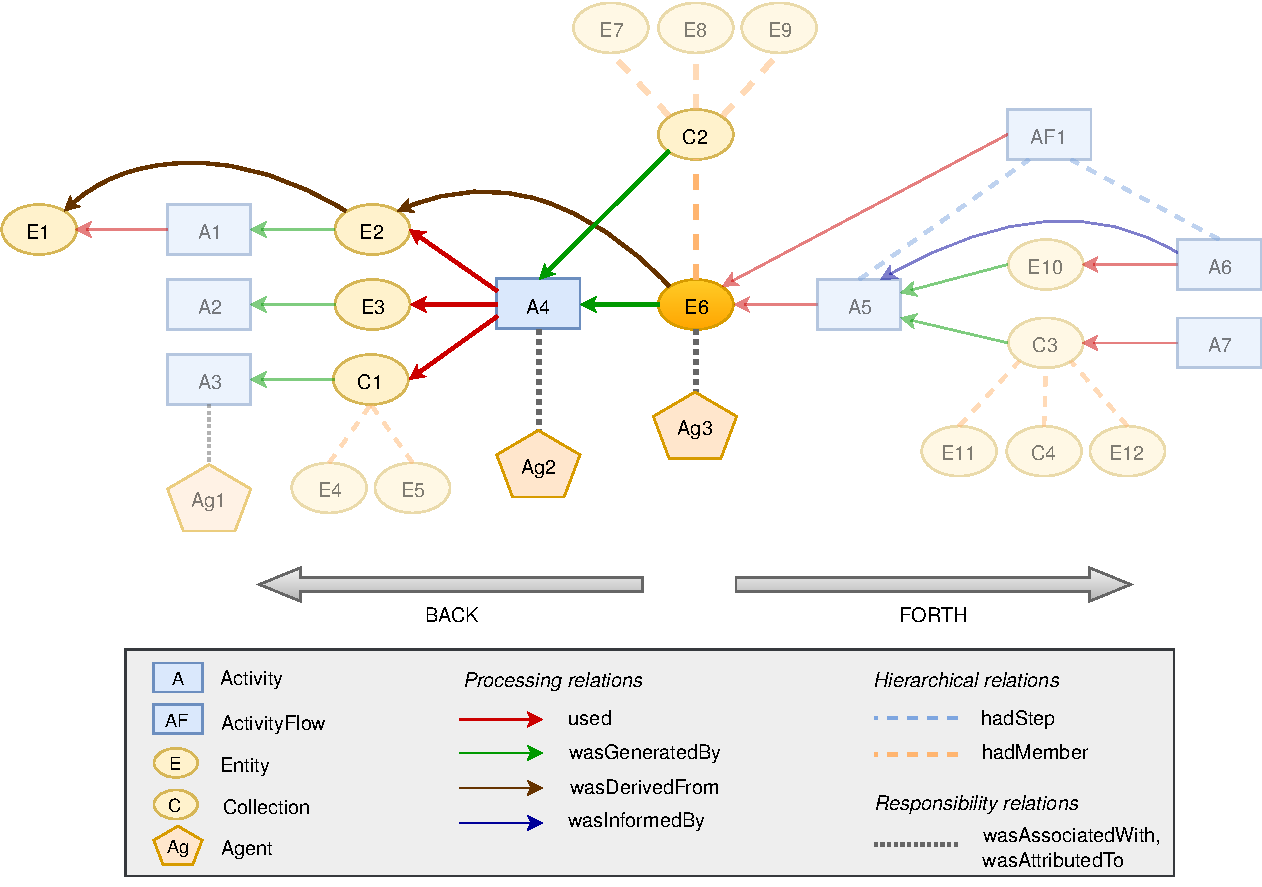
\includegraphics[width=1.0\textwidth]{provenance-graph-example-depth2.pdf}
\caption{An example provenance graph, highlighting the objects and relations returned from a ProvDAL service with \texttt{ID=E6} and \texttt{DEPTH=2}. The BACK and FORTH values for DIRECTION are only important for the processing relations (solid lines). Hierarchial (dashed) and responsibility (dotted) relations are only followed ``upwards'' (to collection/activityFlow) and towards agents by default (unless the optional parameters MEMBERS, STEPS and/or AGENT are set to true.}
\label{fig:provenance-graph-example}
\end{figure}




\paragraph{MEMBERS, STEPS}
The provenance data model defines the hierarchical relations \emph{hadMember} for entity collections and \emph{hadStep} for activityFlows. If a node belongs to a collection or activityFlow, these relations shall be returned as well, independent of the specified tracking direction.
If someone is interested in more details and wants to follow the \emph{members} of an entity collection or the \emph{steps} of an activityFlow, these can be included by setting the optional parameter MEMBERS or STEPS to true, respectively. The default is false. As detailed in DALI, the values 1 and 0 are equivalent to true and false.

\paragraph{AGENT}
By default, it is recommended to stop any further tracking at an agent node, unless an additional optional parameter AGENT is set to true. Note that this means that the request for any agent will always return just the agent node itself and nothing else, unless AGENT=true is used. An example request if one wants to know which entities and activities an agent has influenced could look like this:\\\texttt{\{provdal-base-url\}?ID=org:rave\&AGENT=true\&DEPTH=1}.\\
\texttt{DEPTH=1} is used here in order to avoid following the found entities and activities any further (can be omitted, since this is the default for DEPTH).
\newline
%\comment{Maybe it's better to use DEPTH and DIRECTION instead of FORWARD and BACKWARD. Reason: if a service just implements the backward direction, then it's weird to call something ``backward'' if there is no ``forward'' as well. DEPTH is also a commonly used word when refering to graphs and numbers of relations.}



A ProvDAL service MUST implement the parameters ID, DEPTH and FORMAT; the remaining parameters are optional.
If a service does not implement the optional parameters, but they appear in the request, then the service should return with an error.
Please note that according to the DALI specification \citep{std:DALI}, the parameter names are case-insensitive, but the parameter values are not. E.g. \texttt{direcion=FORTH} is allowed, but \texttt{DIRECTION=forth} may not work.


\subsubsection{ProvDAL example use cases}
We provide here a few example use cases for ProvDAL in order to show its usefulness in exploring the provenance
of astronomical datasets, processes or the people and projects involved in producing/performing them.

\begin{itemize}
\item The RAVE DR4 release contains a main table with stellar properties for each observation of a star. Given the RAVE observation ID, retrieve the processing steps
for this specific observation result:

	\begin{verbatim}
	{provdal-base-url}?ID=rave:20121220_0752m38_089&DEPTH=ALL
	\end{verbatim}

The result will not only contain the processing steps (activities), but also entities and agents. The important information can be filtered out by a client application (e.g. use voprov Python package). If a W3C tool shall be used, one needs to transform the response into a W3C compliant serialisation (e.g. for loading the result to ProvStore\footnote{https://provenance.ecs.soton.ac.uk/store/} for further processing).

\item Get the direct progenitor of an entity:
	\begin{verbatim}
	{provdal-base-url}?ID=rave:20121220_0752m38_089&DEPTH=1
	\end{verbatim}
	If this request only returns a collection and not any ``backwards'' information about progenitors, then
	one needs to track the collection further, i.e. repeat the request for the collection entity.

\item Get all datasets that were derived from a specific data file in the CTA pipeline:
	\begin{verbatim}
	{provdal-base-url}?ID=cta:df1&DEPTH=ALL&DIRECTION=FORTH
	\end{verbatim}
	By using \texttt{DIRECTION=FORTH} we can track the dataset and where it was used forward.

\item Find all people that were involved in processing a dataset along with their contact data (if available), so that one can ask them for further information.
	\begin{verbatim}
	{provdal-base-url}?ID=ex:e1&DEPTH=ALL
	\end{verbatim}
 	The ProvDAL request is basically the same as in the first example. From the results the agents need to be filtered.
 	Since the response contains the nodes and relations including all their properties, the contact details for the agents are included as well (if they are stored with the service).

\item Retrieve a VOTABLE serialisation of the provenance for an image from a data collection.
	\begin{verbatim}
	{provdal-base-url}?ID=myproject:img1&DEPTH=ALL&FORMAT=PROV-VOTABLE
	\end{verbatim}
	We use the FORMAT keyword here to retrieve a VOTABLE.
\end{itemize}

ProvDAL is meant to be used to retrieve parts of a provenance graph from a provenance web service. It cannot be used to retrieve information based on specific properties, e.g. the creationTime of an entity or a parameter value for an activity. For such cases, a ProvTAP service can be used (see next section).


\TODO{Add paragraph on VOSI-endpoints? (DALI service!)}
